\documentclass[a4paper, 12pt finnish]{article}
\usepackage[finnish]{babel}
\usepackage{graphicx}
\usepackage[utf8]{inputenc}
\usepackage[T1]{fontenc}

\title{Dokumentaatio \\ \large Tietokantasovellus}
\author{Joosua Laakso}
\date{\today}

\begin{document}
\maketitle

\section{Johdanto} 
\subsection{Työn aihe} Työn aiheena on työaikatietokanta. Sovellus on
suunniteltu erityisesti logistiikka-alan käyttöön. Tarkoituksena on, että
logistiikka-alalla työskentelevät autonkuljettajat voisivat paperisten
lomakkeiden täyttämisen sijaan syöttää tiedot työkeikkoihin käyttämästään
ajasta suoraan sovellukseen, jonka pitäisi huomattavasti vähentää 
työnantajan kirjanpitoasioihin käyttämää aikaa, koska tietoja ei enää
tarvitsisi kopioida käsin digitaaliseen muotoon paperisesta muodosta, vaan
ne olisi helposti saatavilla tietokannasta. Järjestelmään voi sisältyä
myös laskun automaattinen luonti, jonka avulla järjestelmään syötettyjen
tietojen perusteella, eli työntekijöiden syöttämien työaikatietojen ja 
työnantajan syöttämien tuntitaksatietojen, voisi luoda laskulomakkeen.

\subsection{Käytetyt tekniikat} Työ toteutetaan Helsingin yliopiston 
Users-palvelinta apuna käyttäen. Työssä käytetään Apache-palvelinsovellusta
sekä PHP-kieltä. Tietokannan hallintajärjestelmänä käytetään
Users-palvelimella paremmin tuettua PostgreSQL-järjestelmää.

\section{Yleiskuva järjestelmästä}
\subsection{Käyttäjäryhmät} Käyttäjät voidaan alustavasti eritellä kolmeen
yleisprofiiliin:
\paragraph{Jokamies} Jokamies viittaa kehen tahansa henkilöön, joka
vierailee tietokantasovelluksen web-sivuilla. Muut käyttäjäryhmät 
sisältyvät myös tähän joukkoon.
\paragraph{Johtaja} Johtoon kuuluvat henkilöt, joille työntekijät
työskentelevät, tai ketkä tahansa henkilöt joiden täytyy päästä käsiksi
työntekijöiden työaikatietoihin. Tähän ryhmään saattavat siis sisältyä myös
esimerkiksi kirjanpitäjät. Johto pääsee käsiksi kaikkiin jonkin
(työ)yhteisön tietoihin.
\paragraph{Työntekijä} Työntekijöihin kuuluvat käyttäjät, jotka syöttävät
työaikatietoja järjestelmään. Työntekijä kuuluu johonkin (työ)yhteisöön
ja kyseisen yhteisön johto näkee syötetyt työaikatiedot. Käyttäjä voi
kuulua sekä johtoon että työntekijöihin.

\subsection{Käyttötapaukset} Kullakin käyttäjäryhmällä on omia
käyttötapauksia. Ohessa on lueteltu näitä käyttötapauksia varustettuna
lyhyillä kuvauksilla. On kuitenkin huomioitava, että kaikkia
käyttötapauksia ei välttämättä kuitenkaan tueta lopullisessa versiossa,
vaan nämä ovat enemmän luonnoksenomaisia.

\paragraph{Jokamies:}
\subparagraph{Järjestelmään rekisteröityminen} Käyttäjän pitää pystyä
rekisteröitymään järjestelmän käyttäjäksi jotta voisi käyttää
järjestelmää. Rekisteröityminen tapahtuu rekisteröitymispalvelua käyttäen.

\paragraph{Johtaja:}
\subparagraph{Yhteisön rekisteröinti} Johtaja on aina johtaja jossain
yhteisössä. Jotta johtajalla olisi jokin yhteisö jota johtaa, täytyy
yhteisön rekisteröinnin olla mahdollista.
\subparagraph{Työaikatietojen katselu} Johtajalle täytyy olla mahdollista
seurata työntekijöiden syöttämiä työaikatietoja.
\subparagraph{Asiakkaan kirjaaminen} Johtajalle täytyy olla mahdollista
kirjata asiakkaan nimi muistiin (käytännössä usein jonkin yrityksen nimi).
Asiakkaaseen liittyy myös tuntitaksa, joka kirjataan myös järjestelmään. 
Asiakkaan poistamisen, sekä asiakkaan tietojen muokkaamisen ja jo 
kirjattujen asiakkaiden tietojen katselun täytyy myös olla tuettuna.
\subparagraph{Työntekijän kutsuminen yhteisöön} Johtajan täytyy pystyä
liittämään työntekijä siihen työyhteisöön järjestelmässä, johon 
työntekijä kuuluu. Työntekijän poistamisen yhteisöstä täytyy myös olla
mahdollista.
\subparagraph{Laskun luonti} Johtajalle olisi hyödyllistä, jos asiakkaan
tuntitaksatietojen sekä työntekijöiden lisäämien työaikatietojen pohjalta
voisi automaattisesti luoda laskun.

\paragraph{Työntekijä:}
\subparagraph{Yhteisöön liittyminen} Työntekijän täytyy pystyä liittyä
yhteisöön, johon johtaja on hänet kutsunut.
\subparagraph{Työaikatietojen syöttäminen} Työntekijän täytyy pystyä
lisäämään työaikatietoja järjestelmään. Työntekijän täytyy pystyä
valitsemaan kenelle asiakkaalle työ suoritettiin valikosta, joka sisältää
ne asiakkaat, joiden tiedot johtaja on syöttänyt järjestelmään. Tärkeää
on kuitenkin, että työntekijä ei pysty näkemään eri asiakkaiden
tuntitaksoja. Toisaalta täytyy kuitenkin olla mahdollista kirjata
järjestelmään jos aika käytettiin johonkin muuhun kun asiakkaalle
työskentelyyn, esimerkiksi auton viemiseen huoltoon tai jos asiakas oli
joku, jota ei löydy valikosta.

\subsection{Käyttötapauskaavio} Ohessa käyttötapaukset kuvattuna
graafisesti.

\begin{figure}[h]
    \centering
    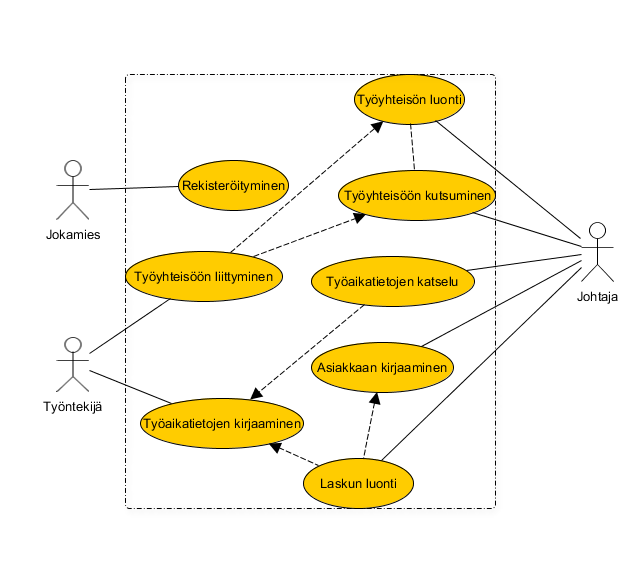
\includegraphics[width=0.9\textwidth]{graafi.png}
    \caption{\small Jos käyttötapaus on riippuvainen jostain toisesta
    käyttötapauksesta, se on merkitty katkoviivanuolella. Kaikki
käyttötapaukset ovat riippuvaisia rekisteröitymisestä, vaikka sitä
ei ole merkitty nuolella.}
\end{figure}


\end{document}
